\newpage
\section{Interesting Techniques}
\hspace{\parindent}
In this section, some techniques that, although not necessarily all of them have been used in the TSEngine, could prove to be beneficial to know and implement when coding a game or graphics engine.

\subsection{Frustum Culling}
\hspace{\parindent}
Frustum culling is a technique used in graphics programming that makes sure that the objects  not visible to camera are not included in the rendering process. As a result, it usually brings great performance improvement, especially in scenes with  complex geometry or numerous objects.
\begin{figure}[H]
    \begin{center}
    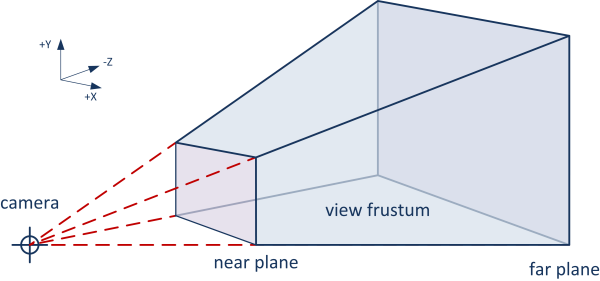
\includegraphics[width=0.8\textwidth]{figures/VisualCameraFrustum.png}
    \end{center}
    \caption{What is view frustum, image from \textit{LearnOpenGL} \cite{learnopengl} }
\end{figure}
As one can see in the image above, to implement frustum culling, the first step is to find six planes that create the boundaries of the view frustum. Objects that lie completely outside the view frustum are not visible to the camera and therefore can be removed from the rendering process. To efficiently determine which object lay completely outside of the six-sided pyramid created by the planes,

\subsection{Entity Component System}
\label{sec:theory_ecs}
\hspace{\parindent}
Entity component system, or ECS for short, is a technique widely used in game engines that has gained great popularity in recent years. This game development architecture offers several benefits over traditional object-oriented programming approaches, making it an attractive choice for game developers, and it was also implemented in TSEngine. The basic idea behind the ECS is to separate the data from its desired behavior and modifications. It is achieved using three types of objects: entities, which essentially are containers for components grouping them together in a way that is readable for a human, components - structures containing all the data, and systems - methods taking all the components of the same type that interact with each other, and achieving some result with it. 

The main advantage of such architecture, is that it is data oriented, focusing on efficient data access and manipulation. It is achieved by storing all components of the same type, near each other in the memory cache, allowing for faster access to them when doing calculations by systems. Another advantage of ECS for many programmers is that it is easily readable and maintainable, allowing for easier development and debugging.

As the entity component system have been used in TSEngine, the following image, representing some implemented code, presents the basic idea behind ECS:
\begin{figure}[H]
  \begin{center}
    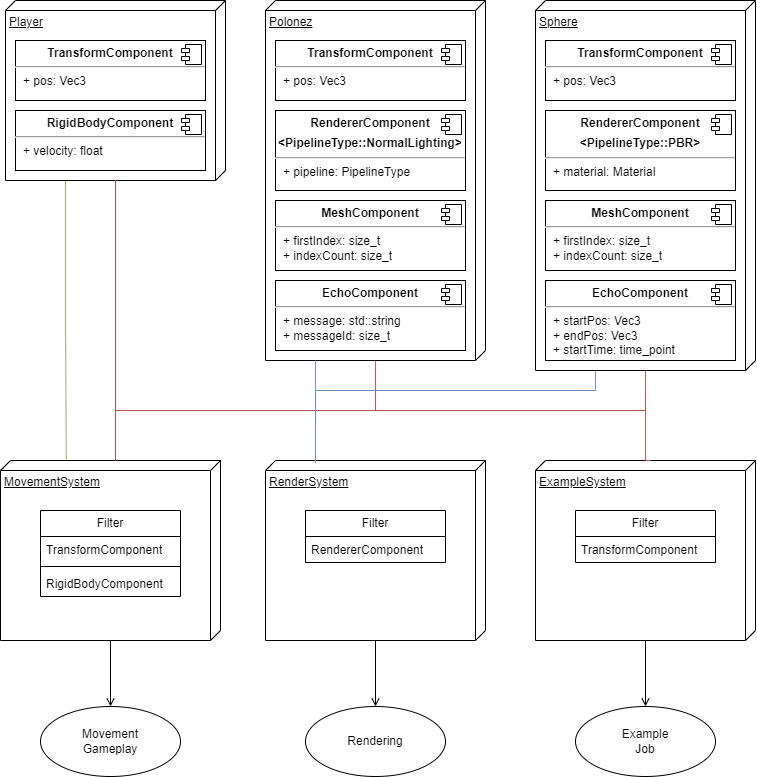
\includegraphics[width=0.8\textwidth]{ecs.png}
  \end{center}
  \caption{ECS in work}
\end{figure}
In this example we have three entities: Player, Polonez and Sphere. Each one has some components assigned to it, and each component can also be assigned to a system that governs it. Taking a closer look at the Movement system, one can see, that to work, it needs a Transform and RigidBody components. When the movement system is invoked, it looks for all such components and uses them to simulate movement. The only entity that has a RigidBody component is Player, and it also has a Transform component, so, when invoked, the Movement system takes Player's RigidBody and Transform components and works with their data, changing their values as the result. The exact details of the implementation of ECS in TSEngine can be found in the section \hyperref[sec:code_ecs]{\ref*{sec:code_ecs} Entity Component System}

\subsection{Reflection System}
\label{sec:refl}
\hspace{\parindent}

\subsection{Deferred vs Forward Rendering}
\label{sec:defer_vs_forward}
\hspace{\parindent}


\newpage
\section{Creation of 3D World Immersion}
\hspace{\parindent}
One might be curious how, from a collection of points, it is possible to create a 3D image. The most important aspect of creating a 3D image on 2D space is perspective. It is achieved thanks to the model, view and projection matrices
\begin{equation}
MVP
\label{mvpequation}
\end{equation}

In some VR devices, because there are two screens for each eye, the matrix has 2 view and projection matrices: 

\begin{equation}
MV[2]P[2]
\label{mvp2equation}
\end{equation}

%For simplicity of explanation, model matrix will be omitted, as it is not always necessary to use it, its main use is to track the object own position in respect to its parent.
The most important matrix to achieve chosen perspective is the projection matrix. It can be different depending on the perspective one would like to achieve, but two most used ones are orthographic projection matrix used for 2D and the matrix for 3D that will be further discussed - perspective projection matrix:

\begin{equation}
\begin{bmatrix}
Orthographic\\
Projection \\
Matrix
\end{bmatrix} 
*
\begin{bmatrix}
X\\
Y\\
Z\\
1\\
\end{bmatrix} 
% \]
\text{ and }
% \[
\begin{bmatrix}
Perspective\\
Projection \\
Matrix
\end{bmatrix} 
*
\begin{bmatrix}
X\\
Y\\
Z\\
1\\
\end{bmatrix}
\label{projectionmatrices}
\end{equation}

To create correct perspective, some additional variables are needed. Due to the fact that nowadays the screens have different proportions, it is vital to have a way to take this into account when creating projection matrix. The solution is to measure the aspect ratio and to scale the rest of the values by it, the aspect ratio of the display device is defined as:

\begin{equation}
a=\frac{h}{w}
\label{aequation}
\end{equation}

Next, we need to consider the way that both field of view and distance of the object from the viewer affect the scale of the visible object. The bigger the field of view, the smaller the object should appear, and the smaller the distance  between the object and viewer, the larger it should appear.
\begin{figure}[H]
  \begin{center}
  
\includegraphics[width=0.3\textwidth]{figures/f_factor.png}  
  \end{center}
  \caption{calculating the f factor}
\end{figure}

 As one can see in the previous image, to deal with the both values at once, we can calculate the tangent of $\theta/2$ angle, and the received value is called factor f, which by we scale the matrix.

\begin{equation}
f=\frac{1}{tan(\theta / 2)}
\label{fequation}
\end{equation} 

Now, to properly convert the image to the screen space as a matrix, we need to also normalize the value of z's. To do so two values are needed: zfar which basically is the maximum distance that objects can be visualized, and znear - the closest possible value that objects can be visualized. 

\begin{figure}[H]
  \begin{center}
  
\includegraphics[width=0.3\textwidth]{figures/normalizing_z.png}  
  \end{center}
  \caption{calculating the f factor}
\end{figure}

The values are then used to calculate the new, normalized value of the z coordinate, let's call it $\lambda$, according to the equation:
\begin{equation}
\lambda=\frac{zfar}{zfar - znear)}
-
\frac{zfar * znear}{zfar-znear}
\label{zequation}
\end{equation} 

Now that we have gathered all the necessary elements, finally, we can go through the process of normalizing the device space.

At first, we begin with coordinates:

\[
\begin{bmatrix}
x\\
y\\
z\\
\end{bmatrix}
\]
which we then convert to screen space with calculated values 
\[
\begin{bmatrix}
afx\\
fy\\
\lambda z-\lambda znear\\
\end{bmatrix}
\]
next we do a simple perspective divide $x/z\ y/z\ z/z$, and as the end result we should be left with normalized device space such as the one in the image below.


\begin{figure}[H]
  \begin{center}
  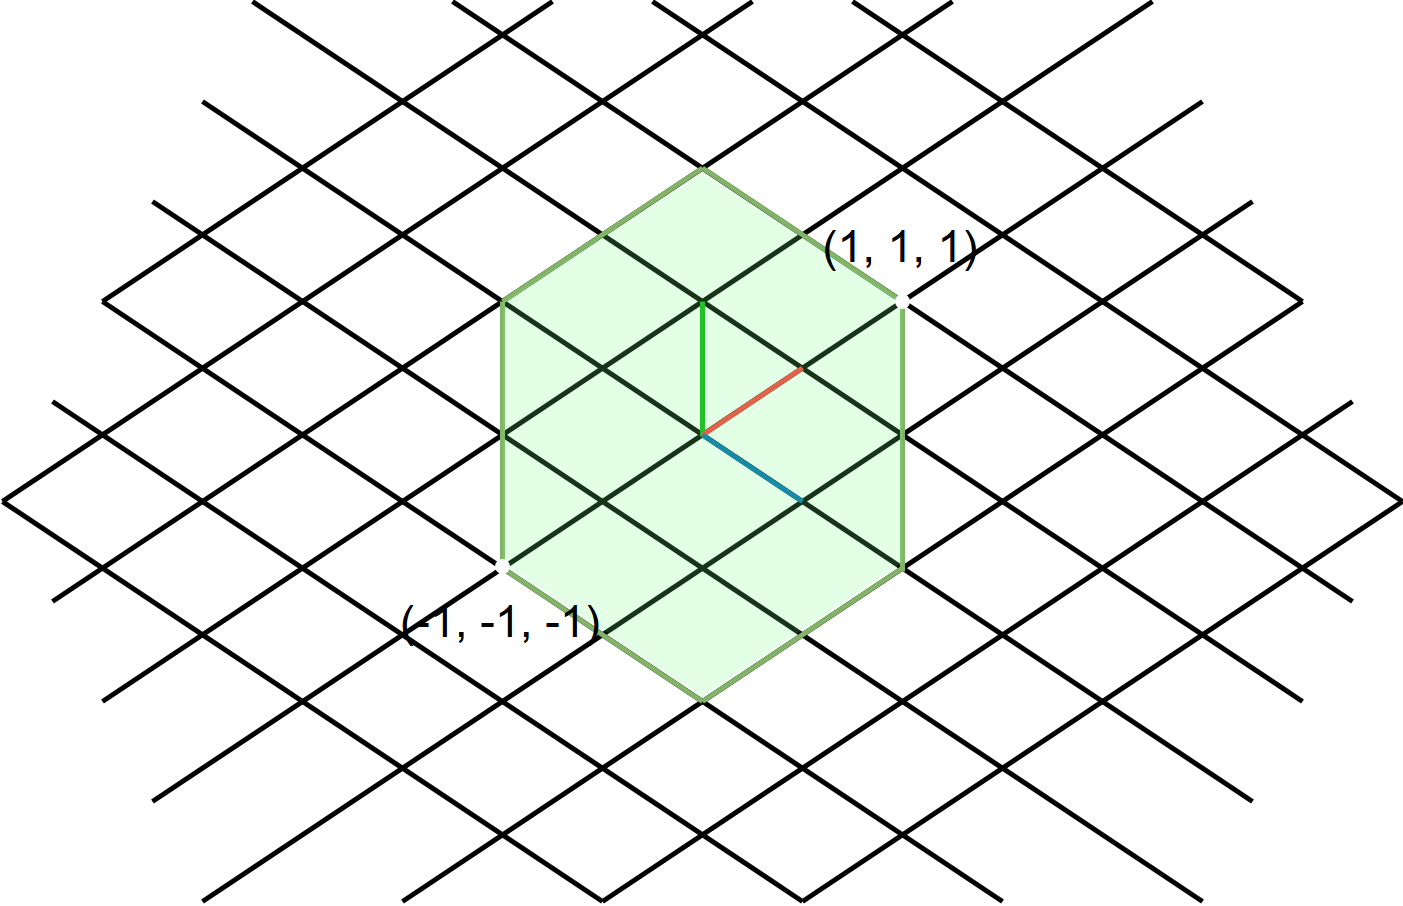
\includegraphics[width=0.5\textwidth]{figures/space.png}  
  \end{center}
  \caption{Normalized device space}
\end{figure}

Now that the theory behind the projection matrix is explained, one question remain: how to implement it? In programming, so as not to lose any values, it is necessary to implement the projection matrix as a four by four matrix: 
\begin{equation}
\begin{bmatrix}
(\frac{h}{w})(\frac{1}{tan(\theta/2)}) & 0 & 0 & 0\\
0 & (\frac{1}{tan(\theta/2)}) & 0 & 0\\
0 & 0 & \frac{zfar}{zfar - znear)} & -\frac{zfar * znear}{zfar-znear}\\
0 & 0 & 1 & 0
\end{bmatrix} 
*
\begin{bmatrix}
X\\
Y\\
Z\\
1\\
\end{bmatrix} 
\label{projectionmatrixequation}
\end{equation} 


An example of view matrix with camera placed at: 10 5 10:
\[
\begin{bmatrix}
1 & 0 & 0 & -10\\
0 & 1 & 0 & -5\\
0 & 0 & 1 & -10\\
0 & 0 & 0 & 1\\
\end{bmatrix} 
\]

\newpage
\section{Software Testing}
\label{sec:testing}
\hspace{\parindent}
Software development can be a lengthy and convoluted process, so to assure the quality of the project and to prevent hidden errors from disturbing workflow, it is necessary to test the code. There are various methodologies used in the process of software testing, and it is of great importance to be aware of them and best situations to use each of them.
\subsection{Unit Tests}
\hspace{\parindent}
One of the simplest ways for programmers to test their code in development is to use unit tests. This method of software testing focuses on validating the functionality of a single unit or component of the tested code. Usually, unit test are written by the same person or team that coded the feature right after finishing said feature. The main advantage of using unit tests is the ease of implementation and high ratio of finding bugs that are quite obvious but potentially very dangerous for future production. As this type of testing was used in the development of TSEngine, the exact way it was used is described in \hyperref[sec:tests]{\ref*{sec:tests} Tests} section.

\subsection{Smoke Tests}
\hspace{\parindent}
Smoke testing, also known as sanity testing or build verification testing, is a methodology that focuses on quickly checking whether the software has any obvious errors or whether the most basic functionalities work properly. This type of testing is the most suited to determine if the software is ready for more in depth tests, or if it is ready for development of the new features. Although this way of testing was used in the development of TSEngine, there is not any documentation of the process, as it was always a simple check after implementing a new feature.

\newpage
\section{Teamwork}
\label{sec:teamwork}
\hspace{\parindent} % TODO: place here any image to make it more funny like that devops from we used for presentation

As in all projects that involve multiple people, it is crucial to develop a way to share each person's work and to have access to previous iterations of the software. Nowadays, it is of great ease with the emergence of version control systems such as Git or Perforce. 

The TSEngine uses Git and furthermore GitHub to accommodate this problem, as described in detail in \hyperref[sec:scv]{\ref*{sec:scv} Source Control Version} section. Git is released under the open source license -  GNU General Public License version 2.0, and as an open source software is widely used in many sites and platforms: GitHub, GitLab or Bitbucket to name the most popular ones, but there are many more developed and used to accommodate specific needs and preferences of the developers.

Another popular method of version control, although not used in the development of TSEngine, is Perforce, now rebranded as Helix Core. It is a powerful tool used mainly in larger projects by AAA game developers, visual effects studios and semiconductor companies. When using Perforce, one must note that it is proprietary software of Perforce Software, Inc. and is free to use only in teams up to 5 users and 20 workspaces. Perforce is more focused on changing files and is better suited than git when dealing with binary files. As always, in software development it is important to choose the correct tool for the project, and it can make the process of development much easier.

The labor of work we put into the project is explained in \hyperref[]{\ref*{sec:labor} Division Of The Labor}.



